\documentclass[./00PhotoBox.tex]{subfiles}
\graphicspath{{\subfix{./img/}}}

\begin{document}

\chapter{Bedienungsanleitung}
\label{ch:Bedienungsanleitung}

\begin{figure}[ht]
    \centering
    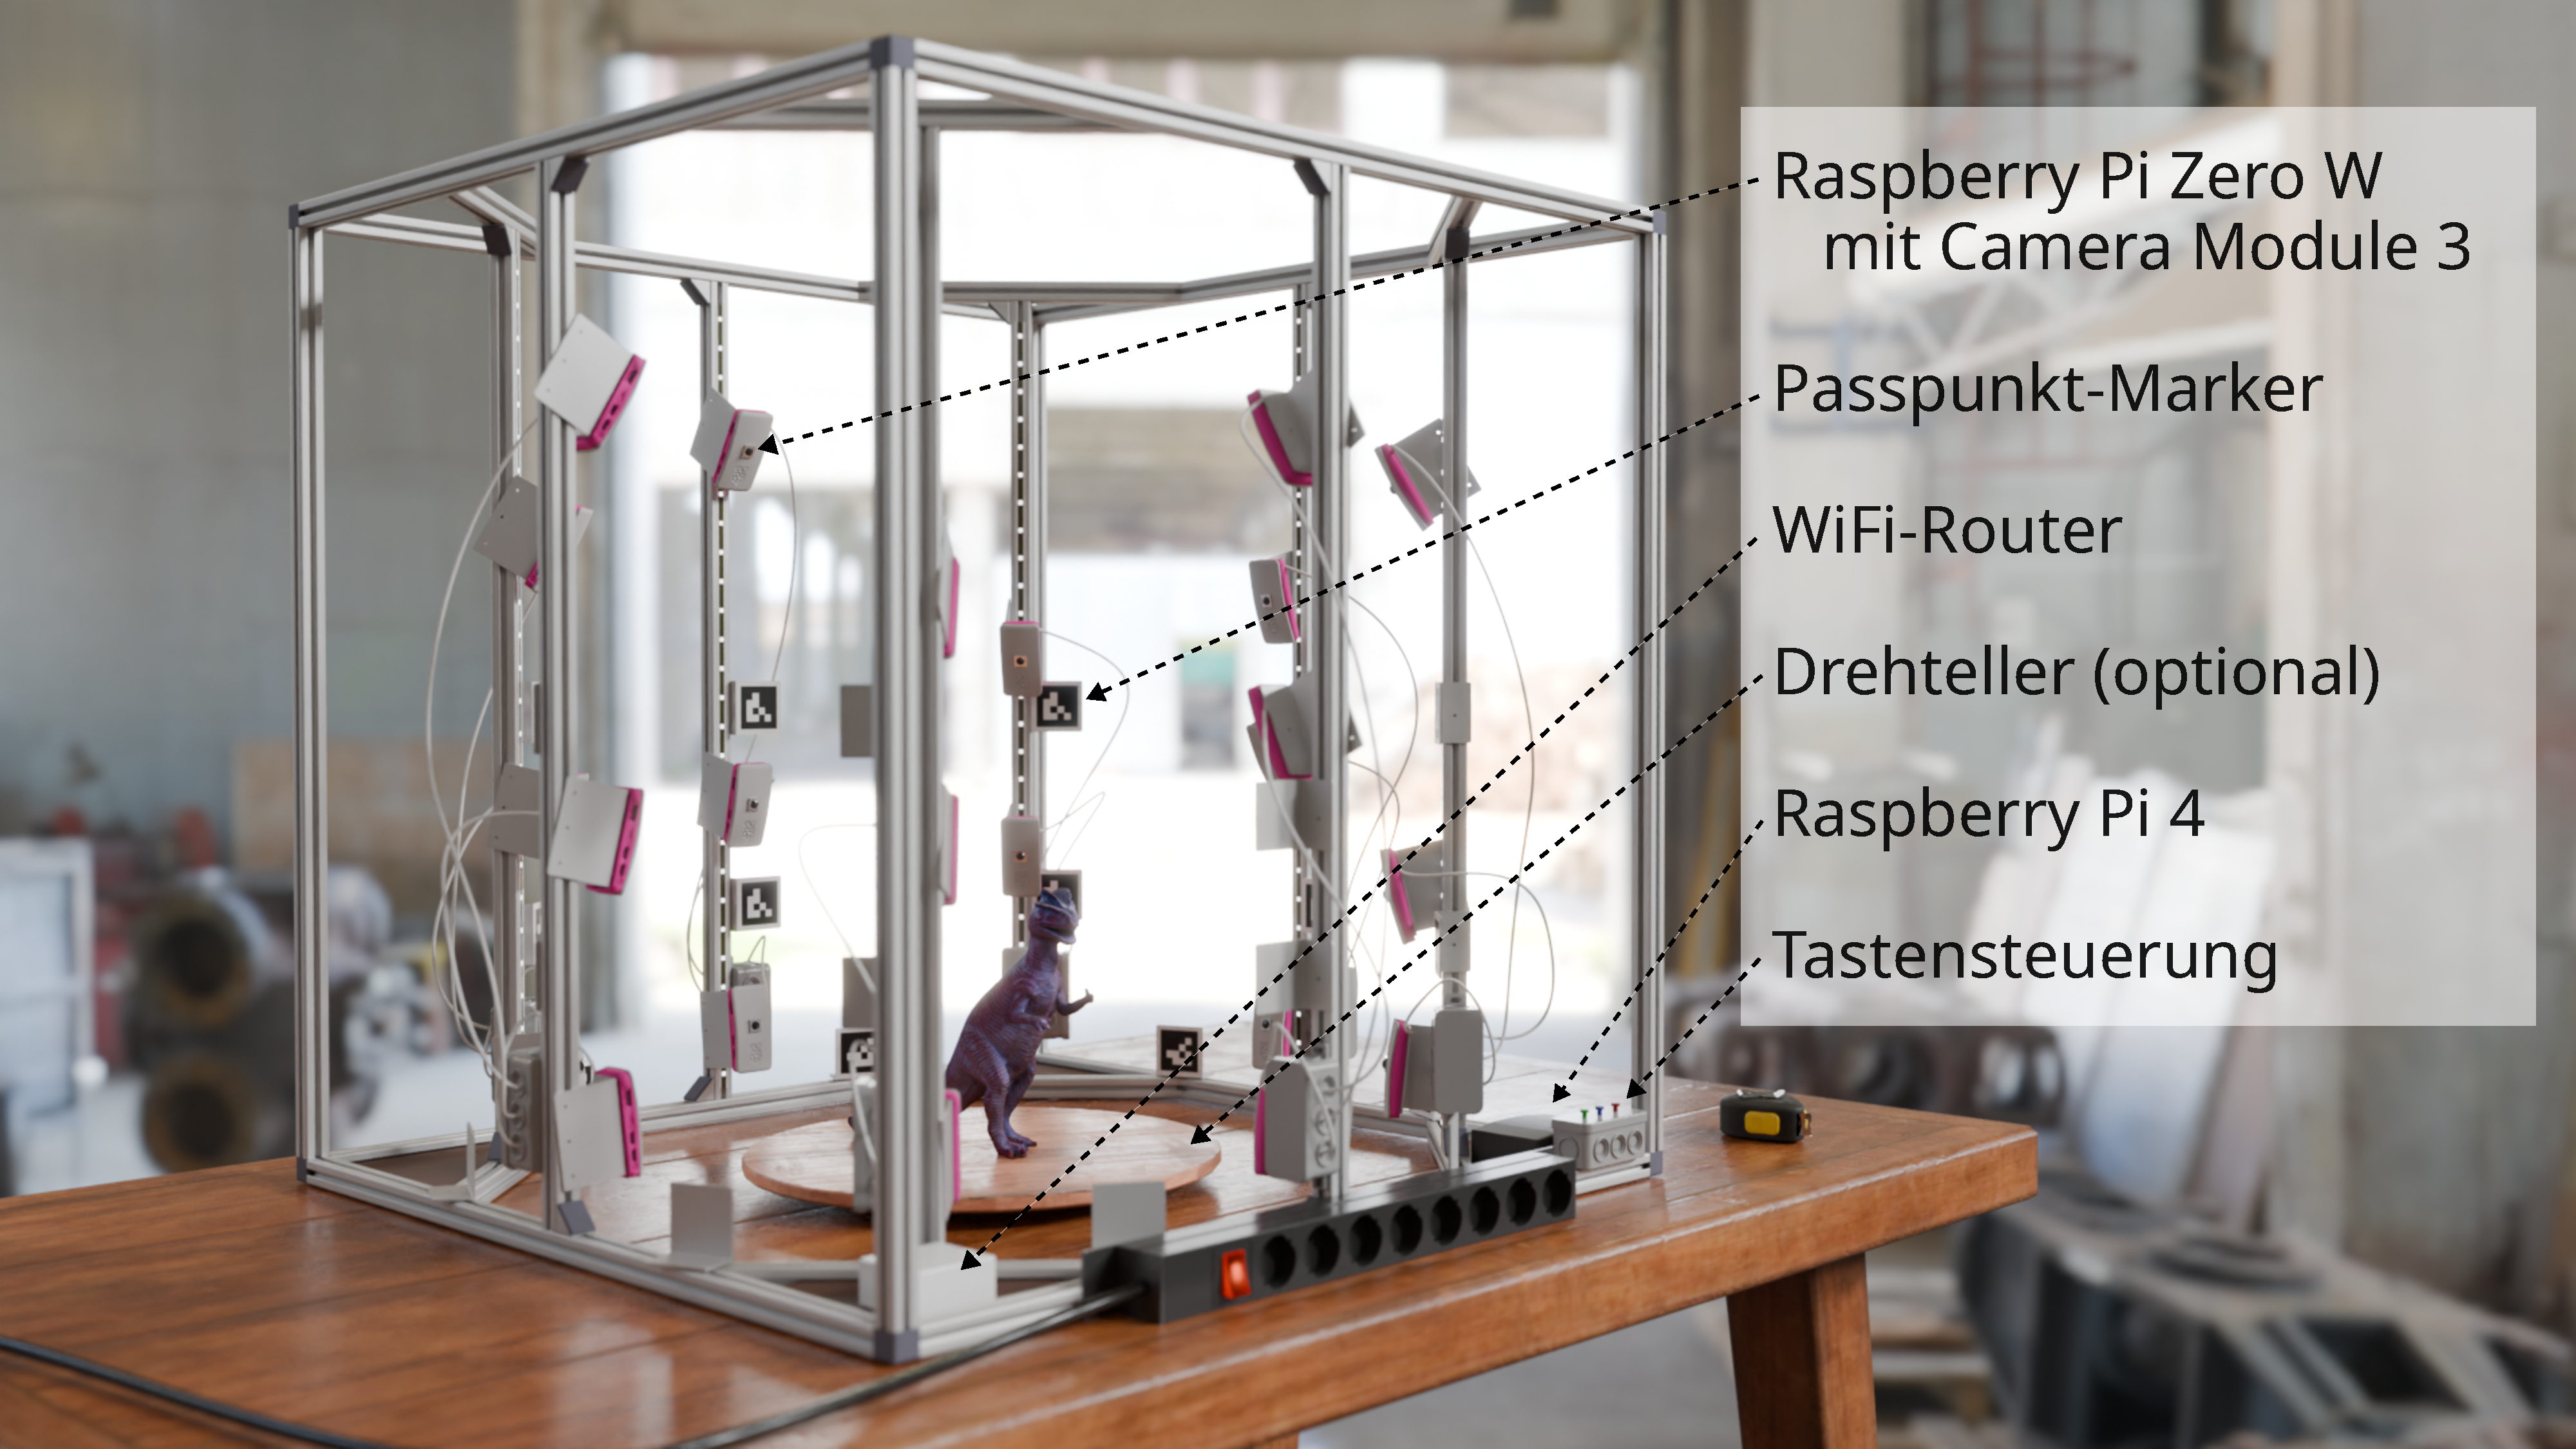
\includegraphics[width=1\textwidth]{./img/9_anleitung/komponenten.pdf}
    \caption{Überblick über das System und seine Komponenten (vereinfachtes Rendering)}
    \label{img:komponenten}
\end{figure}

\section{Anwendungsbereich}
Ziel des Systems ist es, 3D-Modelle von Objekten bis zu einer Größe von \SI{40}{\centi\metre} Durchmesser zu erstellen. Die Bedienung soll dabei möglichst einfach und selbsterklärend sein, um auch Laien die Möglichkeit zu geben, das System zu bedienen.

\section{Menü-Struktur der Weboberfläche}
\subsection{\foreignlanguage{british}{Capture Data}}
\begin{itemize}
    \item \textbf{\foreignlanguage{british}{Photo}} - au\-to\-ma\-tische Aufnahme eines Bildes pro Kamera
    \item \textbf{\foreignlanguage{british}{Focus-Stack}} - au\-to\-ma\-tischer Fokus-Stack mit fünf Bildern pro Kamera
    \item \textbf{\foreignlanguage{british}{Detect ArUco}} - au\-to\-ma\-tische Erkennung von ArUco-Markern
    \item \textbf{\foreignlanguage{british}{Autofocus}} - au\-to\-ma\-tische Fokussierung auslösen
\end{itemize}

\subsection{\foreignlanguage{british}{View Data}}
\begin{itemize}
    \item \textbf{\foreignlanguage{british}{Overview}} - Übersicht über alle Kameras
    \item \textbf{\foreignlanguage{british}{Preview}} - Vorschau eines Bildes und Möglichkeit, Einstellungen auszuprobieren
    \item \textbf{\foreignlanguage{british}{Photo-Download}} - Download der Bilder
    \item \textbf{\foreignlanguage{british}{ArUco-Marker-Coordinates}} - Anzeige und Eingabe der Koordinaten der ArUco-Marker
    \item \textbf{\foreignlanguage{british}{Detected ArUco-Marker}} - Anzeige der Bildkoordinaten der erkannten ArUco-Marker
\end{itemize}

\subsection{\foreignlanguage{british}{Status}}
\begin{itemize}
    \item \textbf{\foreignlanguage{british}{Search}} - Anzeige der System-Informationen
    \item \textbf{\foreignlanguage{british}{Test}} - Anzeige der Kamerastatus
    \item \textbf{\foreignlanguage{british}{Light/Status}} - Umschalten zwischen Beleuchtung und Statusmeldung
\end{itemize}

\subsection{\foreignlanguage{british}{System-Control}}
\begin{itemize}
    \item \textbf{\foreignlanguage{british}{Configuration}} - Einstellungen für Belichtung und Beleuchtung
    \item \textbf{\foreignlanguage{british}{Pause/Resume}} - Pausieren und Starten der Kameras
    \item \textbf{\foreignlanguage{british}{Update}} - Update der Software
    \item \textbf{\foreignlanguage{british}{Restart}} - Neustart der Software
    \item \textbf{\foreignlanguage{british}{Shutdown}} - Herunterfahren des Systems
    \item \textbf{\foreignlanguage{british}{Reboot}} - Neustart des Systems
\end{itemize}


\section{Inbetriebnahme}
Beim Aufstellen ist darauf zu achten, dass sich keine stärkeren seitlichen Lichtquellen um das System herum befinden, wie beispielsweise Fensterflächen. Diese könnten die Belichtung der Bilder beeinflussen und so die Qualität der 3D-Modelle negativ beeinflussen. Gegebenenfalls muss durch die Stoffhülle oder andere Maßnahmen für Verschattung oder Streuung des Lichtes gesorgt werden.

Die Berechnung des 3D-Modelles erfolgt auf einem externen Rechner. Dafür kann wahlweise Agisoft Metashape oder OpenDroneMap (NodeODM) genutzt werden. Die entsprechende Software sowie eine Java-Laufzeitumgebung müssen auf dem Rechner installiert sein und die Bilder müssen auf diesen übertragen werden. Die Übertragung kann au\-to\-ma\-tisch über eine Netzwerkverbindung oder manuell per USB-Stick erfolgen. Für die au\-to\-ma\-tische Übertragung muss die mitgelieferte Verbindungssoftware auf dem Rechner gestartet sein (siehe \autoref{sec:SoftwareEinrichtung}).

Das System startet bei Anschluss an eine Stromversorgung selbstständig. Da die Gefahr besteht, dass die kamerasteuernden Raspberry Pi Zero Daten verlieren, wenn die Stromversorgung unterbrochen wird, sollte das System immer ordnungsgemäß heruntergefahren werden und auf eine zuverlässige Stromversorgung geachtet werden.
Das Abschalten erfolgt durch langes Drücken auf den roten Taster. Das System fährt dann selbstständig herunter - erkennbar an dem Erlöschen der LEDs der Raspberry Pi Zero und der Beleuchtung - und die Stromversorgung kann getrennt werden.

\section{Software-Einrichtung}
\label{sec:SoftwareEinrichtung}
Die Software zur Steuerung der Kameras und zur Übertragung der Bilder auf den Rechner ist in Java geschrieben. Sie kann unter Linux, Windows und MacOS genutzt werden. Auf dem Rechner muss entsprechend eine Java-Laufzeitumgebung installiert sein. Für die Nutzung von Metashape muss eine Lizenz vorhanden sein und im selben Ordner wie die ausführbare jar-Datei abgelegt werden. Für OpenDroneMap muss die Software in Form von NodeODM auf dem Rechner installiert sein. Alternativ kann OpenDroneMap auch auf einem externen Rechner installiert sein, der über das Netzwerk erreichbar ist.

\section{Kalibrierung}
Die letzten Koordinaten der Passpunkte werden im System gespeichert - daher sollten diese möglichst nicht verändert werden. Falls diese dennoch verändert werden, kann das System einzelne Veränderungen berechnen und nutzen. Bei Änderung einer Vielzahl muss das System jedoch extern neu kalibriert werden, beispielsweise durch Bilder mit einer externen Kamera, wodurch dann die Koordinaten der Passpunkte neu bestimmt werden können. Eine Kalibrierung mit Bordmitteln ist nicht möglich.

\section{Durchführung}

\begin{figure}[htbp]
    \centering
    \begin{subfigure}{0.48\textwidth}
        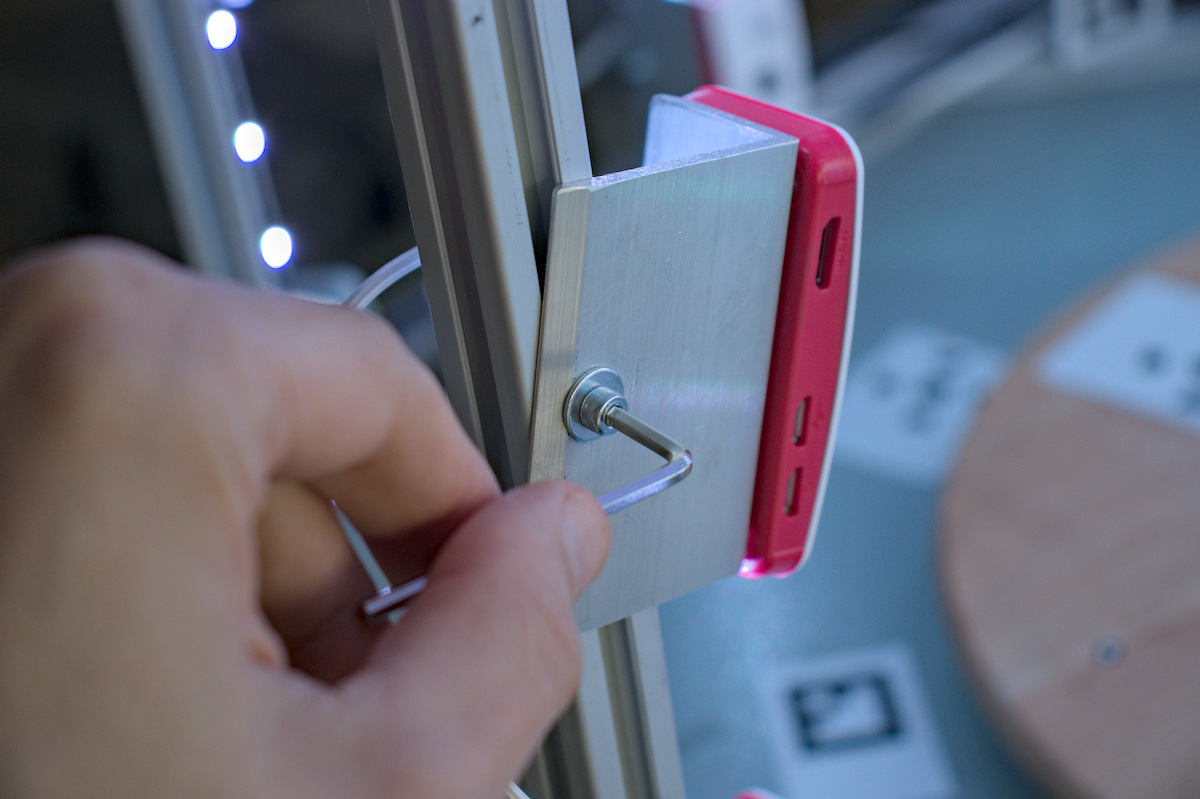
\includegraphics[width=0.95\textwidth]{img/9_anleitung/innensechs.jpg}
        \caption{Nutzung eines Innensechskant-\\schlüssels zur Ausrichtung der\\Kameras}
        \label{img:innensechs}
    \end{subfigure}
    \begin{subfigure}{0.48\textwidth}
        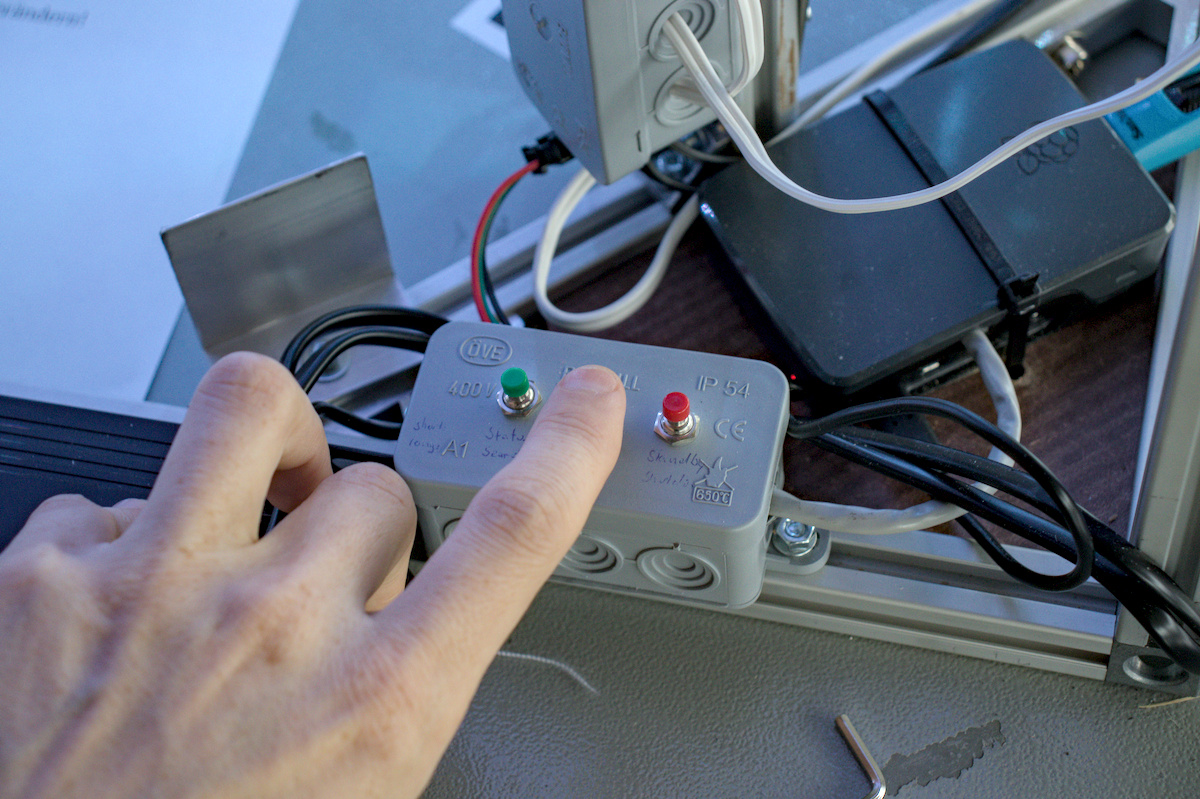
\includegraphics[width=0.95\textwidth]{img/9_anleitung/taster.jpg}
        \caption{Drucktaster zur Steuerung des\\Systems, z.\,B. für die  Bildaufnahme\\~}
        \label{img:taster}
    \end{subfigure}
    \caption{Bedienelemente des Systems}
\end{figure}

Das System wird gestartet, indem die Stromversorgung hergestellt wird. Die Kameras starten selbstständig und die Beleuchtung wird eingeschaltet. Nach kurzer Zeit sollten kurz alle LEDs grün leuchten. Falls nicht, sind einige Kameras nicht erreichbar. Problemlösungen werden im \autoref{sec:Fehlerbehebung} behandelt. Die Kameras können ggf. durch Nutzung einen Innensechskantschlüssels neu ausgerichtet werden (siehe \autoref{img:innensechs}). Eine Bestimmung der neuen Positionen erfolgt selbstständig aus den Passpunkten. Das Objekt wird mittig, ggf. auf einer Erhöhung im Rahmen positioniert. Ab hier trennen sich die Wege je nach verwendetem System. Die Bildaufnahme erfolgt in allen Fällen durch kurzen Druck auf den grünen Taster.

\begin{figure}[htbp]
    \centering
    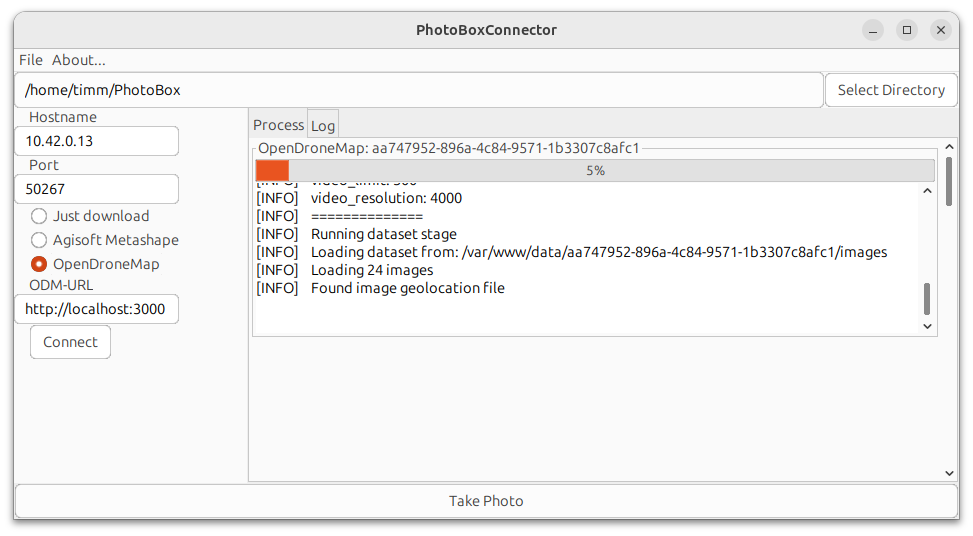
\includegraphics[width=1\textwidth]{./img/5_software/connector_screenshot.png}
    \caption{Screenshot der Connector-Software unter Ubuntu 24.04}
    \label{img:connector}
\end{figure}

\subsection{... mit Netzwerkverbindung}
Der zu verwendende Rechner wird mit dem System per WLAN (bevorzugt) oder Netzwerkleitung verbunden. Die Verbindungssoftware wird gestartet und die IP-Adresse des Systems angegeben. Standardmäßig lautet diese im WLAN 10.0.1.1, per Netzwerkleitung muss die IP von einem DHCP-Server festgelegt werden, beispielsweise in dem der angeschlossene Rechner als DHCP-Server konfiguriert wird. Unter Gnome ist dieses beispielsweise möglich, indem in den Netzwerkeinstellungen die Internetverbindung des PC freigegeben wird.
Anschließend wird die zu nutzende Software ausgewählt und die Verbindung hergestellt.
Nun können die Bilder aufgenommen werden (grüne Taste, \autoref{img:taster}). Die Bilder werden auf den Rechner übertragen und dort in der ausgewählten Software weiterverarbeitet. Der Fortschritt ist in der rechten Hälfte der Verbindungssoftware zu erkennen.

\subsection{... ohne Netzwerkverbindung}
Alternativ können die Bilder ohne angeschlossenen PC aufgenommen werden und später weiter verarbeitet werden. Die Bilder werden in allen Fällen auf dem Raspberry Pi 4, der die gesamte Steuerung übernimmt, gespeichert. Die Bilder können dann von der Website des Raspberry Pi heruntergeladen werden. Auch ist es möglich, einen USB-Stick in den USB-Port des Raspberry Pi 4 vor der Bildaufnahme zu stecken (siehe \autoref{img:usbstick}). Die Bilder werden dann zusätzlich auf den USB-Stick kopiert.

Die Verbindungssoftware unterstützt auch das Laden der Bilder aus einem lokalen Ordner, beispielsweise aus der ZIP der Website oder dem Ordner auf dem USB-Stick. Somit kann dann der weitere Workflow analog zum Workflow mit Netzwerkverbindung durchgeführt und die Bilder weiter verarbeitet werden.

\section{Weiterverarbeitung}
Die Bilder können in der ausgewählten Software weiterverarbeitet werden. Die genaue Vorgehensweise hängt von der Software ab und wird in diesem Abschnitt grob erläutert. Für weitere Informationen hierzu ist die entsprechende Bedienungsanleitung der Software zu konsultieren.

\subsection{Agisoft Metashape}
Sofern in der Schnittstellen-Software aktiviert, wird in Metashape ein Workflow durchgeführt, in dem die Bilder importiert, die Kameras kalibriert, die Passpunkte gesetzt, die Modelle berechnet und exportiert werden. Sofern die Funktion nicht aktiviert wird, wird nur ein Projekt angelegt und die Bilder und Passpunkte importiert. Die weitere Verarbeitung kann dann manuell erfolgen. Hierbei ist darauf zu achten, die Passpunkte zu aktivieren, damit deren Koordinate übernommen wird und der korrekte Maßstab des Modells gewährleistet ist. Anschließend müssten die entsprechenden Schritte manuell durchgeführt werden.

\begin{enumerate}
    \item Haken bei allen Passpunkten und Kameras setzen
    \item \textit{Ablauf / Fotos ausrichten}
    \item Bereich des Modells festlegen
    \item \textit{Ablauf / Punktwolke erzeugen}
    \item ggf. \textit{Ablauf / Mesh erzeugen}
    \item ggf. \textit{Ablauf / Textur erzeugen}
    \item \textit{Exportieren / Modell exportieren} oder \textit{Punktwolke exportieren}
\end{enumerate}

\subsection{OpenDroneMap}
In OpenDroneMap wird ein Prozess gestartet, der die Bilder importiert, die Modelle berechnet und die Modelle exportiert. Hier sind keine weiteren Eingriffe notwendig und möglich.


\section{Wartung}
Software-Updates können zu Inkompatibilitäten führen, daher sollten diese erstmal auf einem zusätzlichen Raspberry Pi ausprobiert werden, bevor diese auf dem System ausgerollt werden. Sofern ein Software-Update durchgeführt werden soll, kann das System per RJ45-Stecker über den Router (siehe \autoref{img:rj45}) mit dem Internet verbunden werden. Anschließend kann das Update der Software über die Weboberfläche durchgeführt werden. Ein Betriebssystemupdate kann per SSH-Verbindung zum Raspberry Pi 4 durchgeführt werden. Hierfür sind die Zugangsdaten am Ende des Dokuments zu finden.

\begin{figure}[htbp]
    \centering
    \begin{subfigure}{0.48\textwidth}
        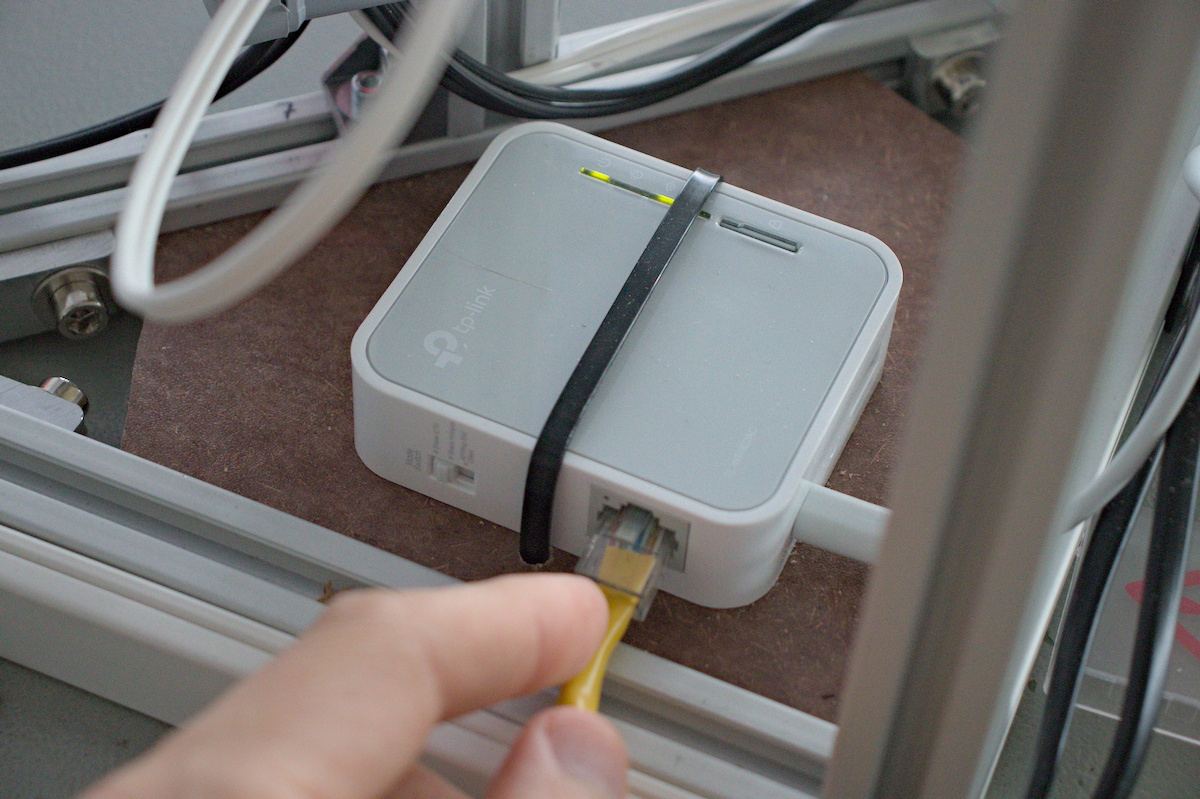
\includegraphics[width=0.95\textwidth]{img/9_anleitung/rj45.jpg}
        \caption{Anschluss eines RJ45-Steckers zur\\Verbindung mit dem Internet\\oder einem PC}
        \label{img:rj45}
    \end{subfigure}
    \begin{subfigure}{0.48\textwidth}
        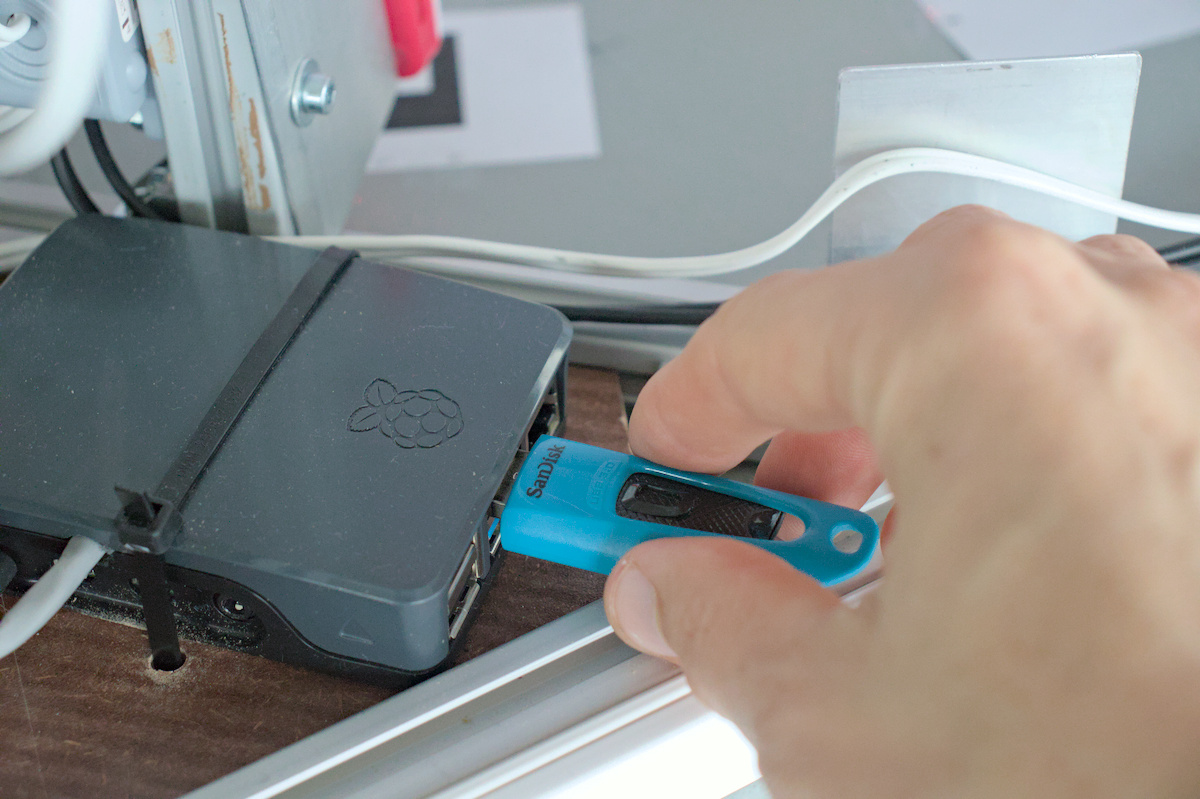
\includegraphics[width=0.95\textwidth]{img/9_anleitung/usbstick.jpg}
        \caption{Anschluss eines USB-Sticks\\ zur Datenübertragung\\~}
        \label{img:usbstick}
    \end{subfigure}
    \caption{Anschlüsse des Systems}
\end{figure}

\section{Fehlerbehebung}
\label{sec:Fehlerbehebung}
\subsection{Kameras sind nicht erreichbar}
Die Kameras sind nicht erreichbar, wenn die LEDs nicht grün leuchten. Dies kann verschiedene Ursachen haben. Als Erstes sollte das System nochmal heruntergefahren werden durch einen langen Druck auf die rote Taste. Anschließend wird die Stromversorgung für einige Sekunden vollständig getrennt und wieder hergestellt. Das System sollte nun neu starten und die Kameras erreichbar sein.

Falls das noch nicht der Fall ist, hilft ein Blick in das Menü des WLAN-Routers. Hier sollten in der Übersicht aller Netzwerkgeräte die 24 Kameras, der steuernde Raspberry Pi 4 und das Gerät, über das der Zugriff erfolgt, aufgezählt sein. Falls das nicht der Fall ist, muss der fehlerhafte Raspberry Pi Zero an einem Display und einer Tastatur angeschlossen werden, um den Fehler zu finden.

Falls der Raspberry Pi im Netzwerk zu finden ist, kann sich per SSH mit dem Raspberry Pi verbunden werden. Zugangsdaten sind die Übersicht am Ende zu entnehmen.

\subsection{Bilder zu hell/zu dunkel}
Je nach Umgebungslicht können die Bilder zu dunkel oder zu hell sein. Im Normalfall sollte die Grundeinstellung mit einem Belichtungswert von +1 zu guten Ergebnissen führen. Falls dies nicht der Fall ist, kann dieses unter \textit{\foreignlanguage{british}{Configuration}} umgestellt werden. Hier kann der Belichtungswert oder die Helligkeit und Lichtfarbe verändert werden.


\section{Zugangsdaten}

\begin{tabular}{|l|l|l|l|}
    \hline
    \textbf{Gerät}    & \textbf{Zugang}     & \textbf{Benutzer} & \textbf{Passwort} \\
    \hline
    WLAN-Netzwerk     & photobox            &                   & photogrammetry    \\
    \hline
    Raspberry Pi 4    & 192.168.1.1:8080    & photo             & box               \\
    \hline
    Raspberry Pi Zero & 192.168.2.1-24:8080 & photo             & box               \\
    \hline
    WLAN-Router       & 192.168.0.1:80      &                   & photobox1         \\
    \hline
\end{tabular}

\biblio
\end{document}